\subsection{Performance of the cluster}\label{sec:benchmark}
Before using the cluster to perform machine learning operations on large amounts of data, a benchmark comparison with a standalone computer will give a good idea of the increase in computing power gained.

To make the comparison, three different files of the sizes 1GB, 5GB, and 10GB.\@ will be generated. They contain unsorted random numbers between $-$2,147,483,646 and 2,147,483,647 which will be treated as strings. To test performance, a word count is performed on the cluster with the specifications seen in \Cref{sec:clustersetup}, and on a standalone computer with:
\begin{itemize}
\item Quad core Intel(R) i7-4500U @ 1.80Ghz 2.40Ghz
\item 8GB RAM
\end{itemize}
where the size of the disk is irrelevant, due to the relatively small sizes of the files. The details of word count was described in \Cref{sec:mapreduce_programming_model}.

\begin{figure}[!htb]
  \centering
    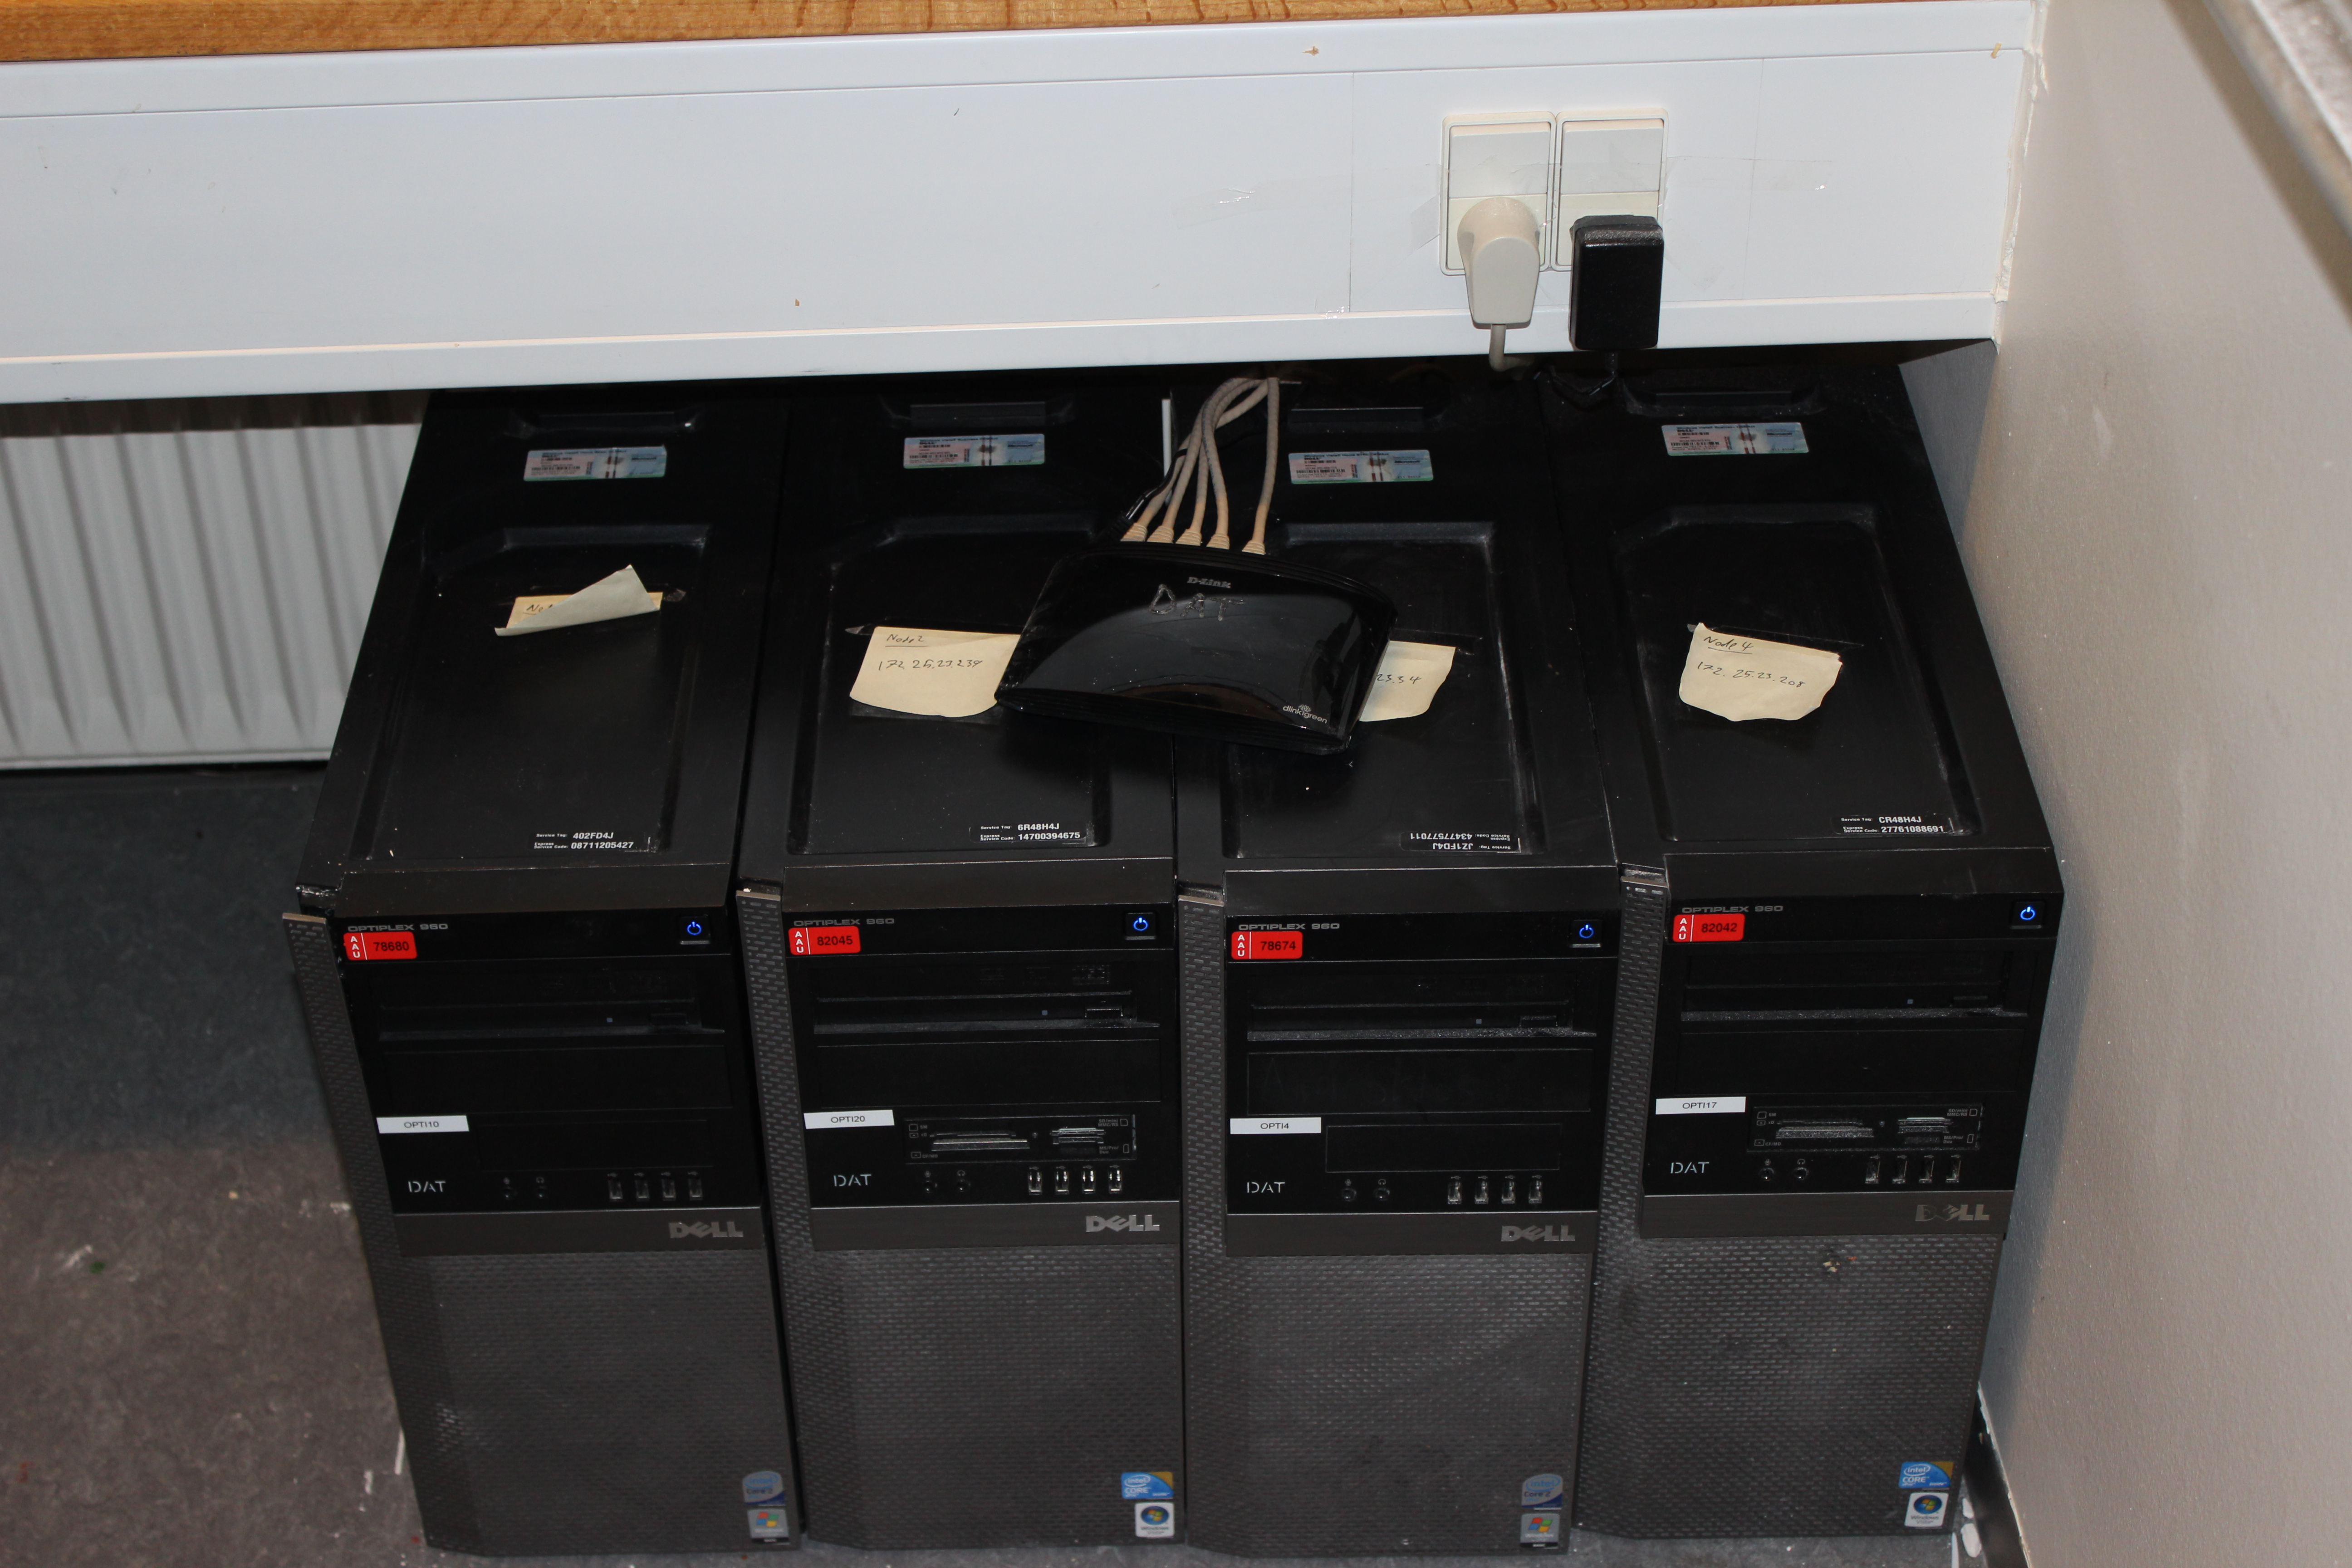
\includegraphics[width=1\textwidth]{img/cluster2.jpg}
  \caption{League of Legends map~\cite{lolmap}}\label{fig:lolmap}
\end{figure}

In \Cref{tab:bench} the time used to perform word count in seconds can be seen, it shows that the cluster can count much faster than a regular standalone computer and this result also makes the cluster comparable to other such distributed systems.

\begin{table}[!htb]
  \centering
  \begin{tabular}{|c|ll|}
    \hline
    File size & Cluster  & Standalone \\
    \hline
    1GB & ? & ? \\
    5GB & ? & ? \\
    10GB & ? & ? \\
    \hline
  \end{tabular}
  \caption{Benchmark tests for the cluster}
  \label{tab:bench}
\end{table}

%%% Local Variables:
%%% mode: latex
%%% TeX-master: "../main"
%%% End:
